\chapter{ESP8266 İle SWD Protokolü Uygulaması}

Bu bölümde, ESP8266 ile SWD protoktolü için sunucu cihaz yapılacaktır. C++ programlama dili ile oluşturulan kodlar ESP8266 için derlenecektir. Bu bölümde [2]'de belirtilen çalışmadan yararlanılmıştır.

SWD protokolünde bulunan üç faz (istek, doğrulama, veri) temelde verinin tek pin (SWDIO) üzerinden saat sinyali ile birlikte, kaydırılarak okunması yada yazılması ile gerçekleştirilir. Burada dikkat edilmesi gereken nokta SWDIO pinin okuma sırasında giriş, yazma sırasında çıkış olarak ayarlanmasıdır.


\section{SWD İstek Verisinin Oluştrulması}

Bir önceki bölümde istek fazı 8 bit uzunluğundaki isteğin hedef cihaza aktarılması olarak bahsetmiştik. Bu istek verisinin öncelikle oluşturulması gerekmektedir. Bu işlemi gerçekleştiren 'packHeader()' C++ kodu Şekil \ref{fig:packHeader} verilmiştir.

\begin{figure}[h]
\centering
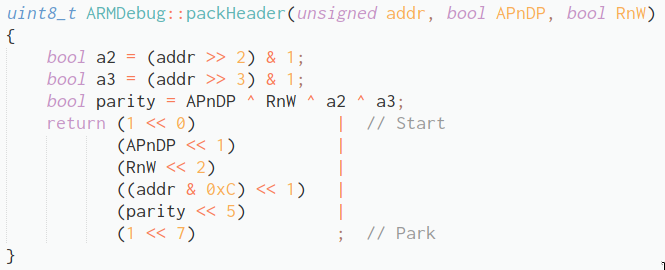
\includegraphics[width=\textwidth]{gorseller/packHeader}
\caption{packHeader() Fonksiyonu}\label{fig:packHeader}
\end{figure}


\section{Verinin Okunması ve Yazılması}

İstek fazının ardından gelen doğrulama ve veri fazı tek hat üzerinden yapılan okuma/yazma işlemidir. SWDIO pini üzerinden okuma işlemini gerçekleyen kod parçası Şekil \ref{fig:wireRead}'de gösterilmiştir. Şekilde gösterilen fonksiyonda bir tane paremetre almaktadır. Bu paremetre okunacak olan verinin bit sayısını temsil etmektedir.
\clearpage
\begin{figure}
\centering
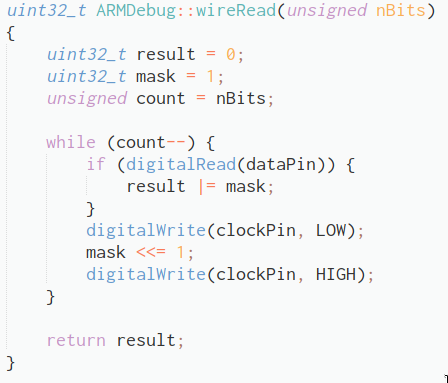
\includegraphics[width=0.6\textwidth]{gorseller/wireRead}
\caption{Okuma İşlemi için C++ Fonksiyonu}\label{fig:wireRead}
\end{figure}

Okunacak bit sayısı kadar tekrarlanan bir döngü içerisinde; SWDIO pini dijital olarak okunur, eğer değer lojik '1' ise sonuç ile maskeleme değişkeni lojik veya (or) işlemine sokulur. Eğer lojik '0' ise maske bir sola kaydırma işlemi yapılır. Döngü sonunda elde edilen sonuç fonksiyon çağrısına geri dönüş yapılır.

Tek pin üzerinde yazma işlemi için oluşturan C++ fonksiyon Şekil \ref{fig:wireWrite}'de gösterilmiştir. Yazma fonsiyonun iki adet parametre almaktadır. Bu parametrelerden biri yazılacak olan veriyi diğer ise verinin kaç bitlik veri olduğunu temsil etmekedir. Yazma işlemi; verinin \acrfull{LSB} öncelikli olarak aktarılması için, 1 ile (0b...00001) maskelenip pine çıkış olarak yazılması ve ardından verinin bir bit sağa kaydırılması, bit sayısı kadar tekrarlamasından oluşan döngüdür.


\begin{figure}[h]
\centering
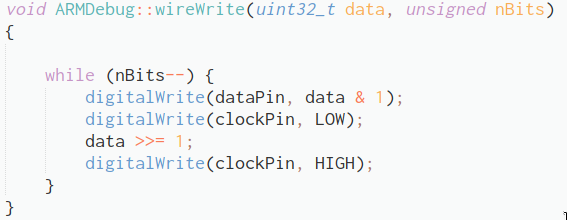
\includegraphics[width=\textwidth]{gorseller/wireWrite}
\caption{Yazma İşlemi için C++ Fonksiyonu}\label{fig:wireWrite}
\end{figure}

Okuma ve yazma fonksiyonları SWD protokolünde bulunan bütün fazlar için ortaktır. İstek fazında 8 bitlik veri yazma işlemi, doğrulama fazında 3 bitlik veri okuma işlemi ve veri fazında hem okuma hem de yazma işlemi yapılır.

Her fazın ardından gelen hat yön değişim periyodu temelde sunucu cihazda SWDIO pini olarak belirlenen pinin giriş yada çıkış olarak ayarlanmasıdır. SWDIO pini istek fazından önce çıkış, doğrulama fazıdan önce giriş, veri fazından önce eğer okuma yapılacak ise hat değişim periyodu uygulanmaz, yazma yapılacak ise hat çıkış olarak ayarlanmalıdır. Hat değişim periyodunu gerçekleyen C++ fonksiyonu Şekil \ref{fig:turnaround}'de verilmiştir.


\begin{figure}[h]
\centering
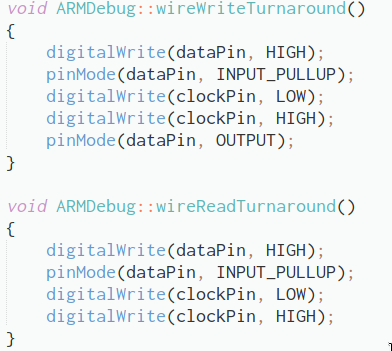
\includegraphics[width=0.7\textwidth]{gorseller/turnaround}
\caption{Yazma ve Okuma İşlemi İçin Hat Yön Değişim Periyodu}\label{fig:turnaround}
\end{figure}


\section{Line Reset}

Bir önceki bölümde SWD bağlantı, reset ve SW-DP portunun şeçimi için gerekli olan işlem sıralarından basettik. Bu işlem sıraları için yazılmış olan kodlar yukarıda belirtilen fonsiyonlar ile gerçekleştirilmiştir. Örnek olarak Şekil \ref{fig:lineReset}' de gösterilmektedir.
\clearpage

\begin{figure}[h]
\centering
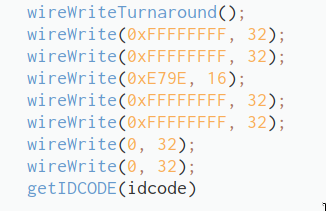
\includegraphics[width=0.7\textwidth]{gorseller/lineReset}
\caption{Yazma ve Okuma İşlemi İçin Hat Yön Değişim Periyodu}\label{fig:lineReset}
\end{figure}

Line reset işlemi için; en az 50 periyotluk '1' verisinin, SW-DP portunun şeçimi için gerekli olan kod '0xE79E' ve tekrar en az 50 bitlik '1' verisi yazılması gerekiyor. 50 bitlik '1' verisi için iki tane 32 bititlik '1' (0xFFFFFFFF) yazılmıştır. Şekilde gösterilen 'getIDCODE()' satırı, protokolün gerekliliği olan fonksiyon çağrısıdır.

